
\documentclass[tikz,border=6pt]{standalone}
\usepackage{tikz}
\usetikzlibrary{positioning}

\definecolor{glass}{RGB}{235,239,244}
\definecolor{etl}{RGB}{82,143,201}
\definecolor{perov}{RGB}{220,112,150}
\definecolor{htl}{RGB}{211,139,65}
\definecolor{metal}{RGB}{105,108,112}

\tikzset{
  layer/.style={
    draw=black!70,
    line width=0.55pt,
    minimum width=5.15cm,
    minimum height=0.62cm,
    align=center,
    font=\sffamily\footnotesize,
    inner sep=2pt
  },
  absorber/.style={
    layer,
    minimum height=1.15cm
  },
  electrode/.style={
    layer,
    text=white
  }
}

\begin{document}
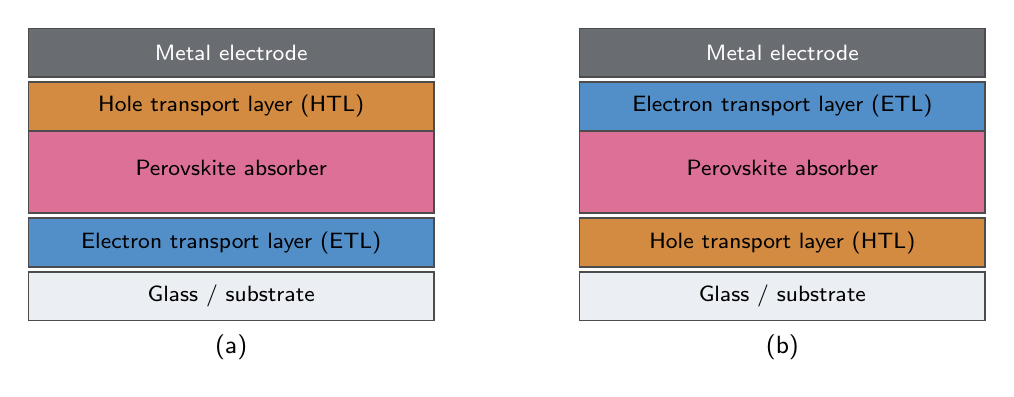
\begin{tikzpicture}[x=1cm,y=1cm]

% ---------------- n-i-p ----------------
\node[layer,fill=glass]    (a1) at (0,0.00) {Glass / substrate};
\node[layer,fill=etl]      (a2) at (0,0.68) {Electron transport layer (ETL)};
\node[absorber,fill=perov] (a3) at (0,1.63) {Perovskite absorber};
\node[layer,fill=htl]      (a4) at (0,2.41) {Hole transport layer (HTL)};
\node[electrode,fill=metal](a5) at (0,3.09) {Metal electrode};

\node[font=\sffamily\small] at (0,-0.65) {(a)};

% ---------------- p-i-n ----------------
\node[layer,fill=glass]    (b1) at (7.0,0.00) {Glass / substrate};
\node[layer,fill=htl]      (b2) at (7.0,0.68) {Hole transport layer (HTL)};
\node[absorber,fill=perov] (b3) at (7.0,1.63) {Perovskite absorber};
\node[layer,fill=etl]      (b4) at (7.0,2.41) {Electron transport layer (ETL)};
\node[electrode,fill=metal](b5) at (7.0,3.09) {Metal electrode};

\node[font=\sffamily\small] at (7.0,-0.65) {(b)};

\end{tikzpicture}
\end{document}
